\documentclass[twoside]{book}

% Packages required by doxygen
\usepackage{calc}
\usepackage{doxygen}
\usepackage{graphicx}
\usepackage[utf8]{inputenc}
\usepackage{makeidx}
\usepackage{multicol}
\usepackage{multirow}
\usepackage{textcomp}
\usepackage[table]{xcolor}

% Font selection
\usepackage[T1]{fontenc}
\usepackage{mathptmx}
\usepackage[scaled=.90]{helvet}
\usepackage{courier}
\usepackage{amssymb}
\usepackage{sectsty}
\renewcommand{\familydefault}{\sfdefault}
\allsectionsfont{%
  \fontseries{bc}\selectfont%
  \color{darkgray}%
}
\renewcommand{\DoxyLabelFont}{%
  \fontseries{bc}\selectfont%
  \color{darkgray}%
}

% Page & text layout
\usepackage{geometry}
\geometry{%
  a4paper,%
  top=2.5cm,%
  bottom=2.5cm,%
  left=2.5cm,%
  right=2.5cm%
}
\tolerance=750
\hfuzz=15pt
\hbadness=750
\setlength{\emergencystretch}{15pt}
\setlength{\parindent}{0cm}
\setlength{\parskip}{0.2cm}
\makeatletter
\renewcommand{\paragraph}{%
  \@startsection{paragraph}{4}{0ex}{-1.0ex}{1.0ex}{%
    \normalfont\normalsize\bfseries\SS@parafont%
  }%
}
\renewcommand{\subparagraph}{%
  \@startsection{subparagraph}{5}{0ex}{-1.0ex}{1.0ex}{%
    \normalfont\normalsize\bfseries\SS@subparafont%
  }%
}
\makeatother

% Headers & footers
\usepackage{fancyhdr}
\pagestyle{fancyplain}
\fancyhead[LE]{\fancyplain{}{\bfseries\thepage}}
\fancyhead[CE]{\fancyplain{}{}}
\fancyhead[RE]{\fancyplain{}{\bfseries\leftmark}}
\fancyhead[LO]{\fancyplain{}{\bfseries\rightmark}}
\fancyhead[CO]{\fancyplain{}{}}
\fancyhead[RO]{\fancyplain{}{\bfseries\thepage}}
\fancyfoot[LE]{\fancyplain{}{}}
\fancyfoot[CE]{\fancyplain{}{}}
\fancyfoot[RE]{\fancyplain{}{\bfseries\scriptsize Generated on Tue Mar 4 2014 04\-:22\-:37 for libgit++ by Doxygen }}
\fancyfoot[LO]{\fancyplain{}{\bfseries\scriptsize Generated on Tue Mar 4 2014 04\-:22\-:37 for libgit++ by Doxygen }}
\fancyfoot[CO]{\fancyplain{}{}}
\fancyfoot[RO]{\fancyplain{}{}}
\renewcommand{\footrulewidth}{0.4pt}
\renewcommand{\chaptermark}[1]{%
  \markboth{#1}{}%
}
\renewcommand{\sectionmark}[1]{%
  \markright{\thesection\ #1}%
}

% Indices & bibliography
\usepackage{natbib}
\usepackage[titles]{tocloft}
\setcounter{tocdepth}{3}
\setcounter{secnumdepth}{5}
\makeindex

% Hyperlinks (required, but should be loaded last)
\usepackage{ifpdf}
\ifpdf
  \usepackage[pdftex,pagebackref=true]{hyperref}
\else
  \usepackage[ps2pdf,pagebackref=true]{hyperref}
\fi
\hypersetup{%
  colorlinks=true,%
  linkcolor=blue,%
  citecolor=blue,%
  unicode%
}

% Custom commands
\newcommand{\clearemptydoublepage}{%
  \newpage{\pagestyle{empty}\cleardoublepage}%
}


%===== C O N T E N T S =====

\begin{document}

% Titlepage & ToC
\hypersetup{pageanchor=false}
\pagenumbering{roman}
\begin{titlepage}
\vspace*{7cm}
\begin{center}%
{\Large libgit++ }\\
\vspace*{1cm}
{\large Generated by Doxygen 1.8.6}\\
\vspace*{0.5cm}
{\small Tue Mar 4 2014 04:22:37}\\
\end{center}
\end{titlepage}
\clearemptydoublepage
\tableofcontents
\clearemptydoublepage
\pagenumbering{arabic}
\hypersetup{pageanchor=true}

%--- Begin generated contents ---
\chapter{Namespace Index}
\section{Namespace List}
Here is a list of all namespaces with brief descriptions\-:\begin{DoxyCompactList}
\item\contentsline{section}{\hyperlink{namespace_git}{Git} \\*Libgit++ }{\pageref{namespace_git}}{}
\end{DoxyCompactList}

\chapter{Hierarchical Index}
\section{Class Hierarchy}
This inheritance list is sorted roughly, but not completely, alphabetically\-:\begin{DoxyCompactList}
\item enable\-\_\-shared\-\_\-from\-\_\-this\begin{DoxyCompactList}
\item \contentsline{section}{Git\-:\-:Commit}{\pageref{class_git_1_1_commit}}{}
\item \contentsline{section}{Git\-:\-:Repo}{\pageref{class_git_1_1_repo}}{}
\item \contentsline{section}{Git\-:\-:Sig}{\pageref{class_git_1_1_sig}}{}
\end{DoxyCompactList}
\item \contentsline{section}{Git\-:\-:Exception}{\pageref{class_git_1_1_exception}}{}
\item \contentsline{section}{Git\-:\-:Object}{\pageref{class_git_1_1_object}}{}
\begin{DoxyCompactList}
\item \contentsline{section}{Git\-:\-:Commit}{\pageref{class_git_1_1_commit}}{}
\item \contentsline{section}{Git\-:\-:Sig}{\pageref{class_git_1_1_sig}}{}
\end{DoxyCompactList}
\end{DoxyCompactList}

\chapter{Class Index}
\section{Class List}
Here are the classes, structs, unions and interfaces with brief descriptions\-:\begin{DoxyCompactList}
\item\contentsline{section}{\hyperlink{class_git_1_1_commit}{Git\-::\-Commit} }{\pageref{class_git_1_1_commit}}{}
\item\contentsline{section}{\hyperlink{class_git_1_1_exception}{Git\-::\-Exception} }{\pageref{class_git_1_1_exception}}{}
\item\contentsline{section}{\hyperlink{class_git_1_1_repo}{Git\-::\-Repo} }{\pageref{class_git_1_1_repo}}{}
\end{DoxyCompactList}

\chapter{File Index}
\section{File List}
Here is a list of all files with brief descriptions\-:\begin{DoxyCompactList}
\item\contentsline{section}{src/\hyperlink{commit_8cpp}{commit.\-cpp} }{\pageref{commit_8cpp}}{}
\item\contentsline{section}{src/\hyperlink{commit_8h}{commit.\-h} }{\pageref{commit_8h}}{}
\item\contentsline{section}{src/\hyperlink{exception_8cpp}{exception.\-cpp} }{\pageref{exception_8cpp}}{}
\item\contentsline{section}{src/\hyperlink{exception_8h}{exception.\-h} }{\pageref{exception_8h}}{}
\item\contentsline{section}{src/\hyperlink{object_8cpp}{object.\-cpp} }{\pageref{object_8cpp}}{}
\item\contentsline{section}{src/\hyperlink{object_8h}{object.\-h} }{\pageref{object_8h}}{}
\item\contentsline{section}{src/\hyperlink{repo_8cpp}{repo.\-cpp} }{\pageref{repo_8cpp}}{}
\item\contentsline{section}{src/\hyperlink{repo_8h}{repo.\-h} \\*Manage repository }{\pageref{repo_8h}}{}
\item\contentsline{section}{src/\hyperlink{signature_8cpp}{signature.\-cpp} }{\pageref{signature_8cpp}}{}
\item\contentsline{section}{src/\hyperlink{signature_8h}{signature.\-h} }{\pageref{signature_8h}}{}
\end{DoxyCompactList}

\chapter{Namespace Documentation}
\hypertarget{namespace_git}{\section{Git Namespace Reference}
\label{namespace_git}\index{Git@{Git}}
}


libgit++  


\subsection*{Classes}
\begin{DoxyCompactItemize}
\item 
class \hyperlink{class_git_1_1_commit}{Commit}
\item 
class \hyperlink{class_git_1_1_exception}{Exception}
\item 
class \hyperlink{class_git_1_1_object}{Object}
\item 
class \hyperlink{class_git_1_1_repo}{Repo}
\begin{DoxyCompactList}\small\item\em Manage repository. \end{DoxyCompactList}\item 
class \hyperlink{class_git_1_1_sig}{Sig}
\end{DoxyCompactItemize}
\subsection*{Functions}
\begin{DoxyCompactItemize}
\item 
void \hyperlink{namespace_git_a278e75304a5420da6ca1611ce9ffddc0}{Throw} (const int \&error)
\item 
git\-\_\-oid \hyperlink{namespace_git_a20e639531f5c04252e0ce86622c2e77e}{oid} (const std\-::string \&sha)
\item 
const std\-::string \hyperlink{namespace_git_a7058573edae76cc2fbafcfe04e13dabc}{oid} (git\-\_\-oid \&oid)
\end{DoxyCompactItemize}


\subsection{Detailed Description}
libgit++ 

\subsection{Function Documentation}
\hypertarget{namespace_git_a20e639531f5c04252e0ce86622c2e77e}{\index{Git@{Git}!oid@{oid}}
\index{oid@{oid}!Git@{Git}}
\subsubsection[{oid}]{\setlength{\rightskip}{0pt plus 5cm}git\-\_\-oid Git\-::oid (
\begin{DoxyParamCaption}
\item[{const std\-::string \&}]{sha}
\end{DoxyParamCaption}
)}}\label{namespace_git_a20e639531f5c04252e0ce86622c2e77e}
\hypertarget{namespace_git_a7058573edae76cc2fbafcfe04e13dabc}{\index{Git@{Git}!oid@{oid}}
\index{oid@{oid}!Git@{Git}}
\subsubsection[{oid}]{\setlength{\rightskip}{0pt plus 5cm}const std\-::string Git\-::oid (
\begin{DoxyParamCaption}
\item[{git\-\_\-oid \&}]{oid}
\end{DoxyParamCaption}
)}}\label{namespace_git_a7058573edae76cc2fbafcfe04e13dabc}
\hypertarget{namespace_git_a278e75304a5420da6ca1611ce9ffddc0}{\index{Git@{Git}!Throw@{Throw}}
\index{Throw@{Throw}!Git@{Git}}
\subsubsection[{Throw}]{\setlength{\rightskip}{0pt plus 5cm}void Git\-::\-Throw (
\begin{DoxyParamCaption}
\item[{const int \&}]{error}
\end{DoxyParamCaption}
)}}\label{namespace_git_a278e75304a5420da6ca1611ce9ffddc0}

\chapter{Class Documentation}
\hypertarget{class_git_1_1_commit}{\section{Git\-:\-:Commit Class Reference}
\label{class_git_1_1_commit}\index{Git\-::\-Commit@{Git\-::\-Commit}}
}


{\ttfamily \#include $<$commit.\-h$>$}

\subsection*{Public Member Functions}
\begin{DoxyCompactItemize}
\item 
void \hyperlink{class_git_1_1_commit_a3540ad2a8f51a895dcb508b95ca8fd39}{update} ()
\item 
void \hyperlink{class_git_1_1_commit_aa759cb4bb4a1ae454d5d76896fabe787}{sig} (const std\-::string \&name, const std\-::string \&email)
\item 
const std\-::string \hyperlink{class_git_1_1_commit_a54d5713f3bff0b54935d55a72c71d4e8}{message} ()
\item 
void \hyperlink{class_git_1_1_commit_a0034dbec5ae88697b8896da8254620de}{message} (const std\-::string \&msg)
\end{DoxyCompactItemize}
\subsection*{Static Public Member Functions}
\begin{DoxyCompactItemize}
\item 
static std\-::shared\-\_\-ptr$<$ \hyperlink{class_git_1_1_commit}{Commit} $>$ \hyperlink{class_git_1_1_commit_ad90040d7ee2670ea170ff071a5bb09bc}{create} ()
\end{DoxyCompactItemize}


\subsection{Member Function Documentation}
\hypertarget{class_git_1_1_commit_ad90040d7ee2670ea170ff071a5bb09bc}{\index{Git\-::\-Commit@{Git\-::\-Commit}!create@{create}}
\index{create@{create}!Git::Commit@{Git\-::\-Commit}}
\subsubsection[{create}]{\setlength{\rightskip}{0pt plus 5cm}std\-::shared\-\_\-ptr$<$ {\bf Commit} $>$ Git\-::\-Commit\-::create (
\begin{DoxyParamCaption}
{}
\end{DoxyParamCaption}
)\hspace{0.3cm}{\ttfamily [static]}}}\label{class_git_1_1_commit_ad90040d7ee2670ea170ff071a5bb09bc}
\hypertarget{class_git_1_1_commit_a54d5713f3bff0b54935d55a72c71d4e8}{\index{Git\-::\-Commit@{Git\-::\-Commit}!message@{message}}
\index{message@{message}!Git::Commit@{Git\-::\-Commit}}
\subsubsection[{message}]{\setlength{\rightskip}{0pt plus 5cm}const std\-::string Git\-::\-Commit\-::message (
\begin{DoxyParamCaption}
{}
\end{DoxyParamCaption}
)}}\label{class_git_1_1_commit_a54d5713f3bff0b54935d55a72c71d4e8}
\hypertarget{class_git_1_1_commit_a0034dbec5ae88697b8896da8254620de}{\index{Git\-::\-Commit@{Git\-::\-Commit}!message@{message}}
\index{message@{message}!Git::Commit@{Git\-::\-Commit}}
\subsubsection[{message}]{\setlength{\rightskip}{0pt plus 5cm}void Git\-::\-Commit\-::message (
\begin{DoxyParamCaption}
\item[{const std\-::string \&}]{msg}
\end{DoxyParamCaption}
)}}\label{class_git_1_1_commit_a0034dbec5ae88697b8896da8254620de}
\hypertarget{class_git_1_1_commit_aa759cb4bb4a1ae454d5d76896fabe787}{\index{Git\-::\-Commit@{Git\-::\-Commit}!sig@{sig}}
\index{sig@{sig}!Git::Commit@{Git\-::\-Commit}}
\subsubsection[{sig}]{\setlength{\rightskip}{0pt plus 5cm}void Git\-::\-Commit\-::sig (
\begin{DoxyParamCaption}
\item[{const std\-::string \&}]{name, }
\item[{const std\-::string \&}]{email}
\end{DoxyParamCaption}
)}}\label{class_git_1_1_commit_aa759cb4bb4a1ae454d5d76896fabe787}
\hypertarget{class_git_1_1_commit_a3540ad2a8f51a895dcb508b95ca8fd39}{\index{Git\-::\-Commit@{Git\-::\-Commit}!update@{update}}
\index{update@{update}!Git::Commit@{Git\-::\-Commit}}
\subsubsection[{update}]{\setlength{\rightskip}{0pt plus 5cm}void Git\-::\-Commit\-::update (
\begin{DoxyParamCaption}
{}
\end{DoxyParamCaption}
)}}\label{class_git_1_1_commit_a3540ad2a8f51a895dcb508b95ca8fd39}


The documentation for this class was generated from the following files\-:\begin{DoxyCompactItemize}
\item 
src/\hyperlink{commit_8h}{commit.\-h}\item 
src/\hyperlink{commit_8cpp}{commit.\-cpp}\end{DoxyCompactItemize}

\hypertarget{class_git_1_1_exception}{\section{Git\-:\-:Exception Class Reference}
\label{class_git_1_1_exception}\index{Git\-::\-Exception@{Git\-::\-Exception}}
}


{\ttfamily \#include $<$exception.\-h$>$}

\subsection*{Public Member Functions}
\begin{DoxyCompactItemize}
\item 
\hyperlink{class_git_1_1_exception_a6e3707a1171cf3b5b2e6e5ec75be1b05}{Exception} (const int error)
\item 
const std\-::string \hyperlink{class_git_1_1_exception_aea19628d8fc5b72abd99f269401acbb6}{message} ()
\end{DoxyCompactItemize}


\subsection{Constructor \& Destructor Documentation}
\hypertarget{class_git_1_1_exception_a6e3707a1171cf3b5b2e6e5ec75be1b05}{\index{Git\-::\-Exception@{Git\-::\-Exception}!Exception@{Exception}}
\index{Exception@{Exception}!Git::Exception@{Git\-::\-Exception}}
\subsubsection[{Exception}]{\setlength{\rightskip}{0pt plus 5cm}Git\-::\-Exception\-::\-Exception (
\begin{DoxyParamCaption}
\item[{const int}]{error}
\end{DoxyParamCaption}
)}}\label{class_git_1_1_exception_a6e3707a1171cf3b5b2e6e5ec75be1b05}


\subsection{Member Function Documentation}
\hypertarget{class_git_1_1_exception_aea19628d8fc5b72abd99f269401acbb6}{\index{Git\-::\-Exception@{Git\-::\-Exception}!message@{message}}
\index{message@{message}!Git::Exception@{Git\-::\-Exception}}
\subsubsection[{message}]{\setlength{\rightskip}{0pt plus 5cm}const std\-::string Git\-::\-Exception\-::message (
\begin{DoxyParamCaption}
{}
\end{DoxyParamCaption}
)}}\label{class_git_1_1_exception_aea19628d8fc5b72abd99f269401acbb6}


The documentation for this class was generated from the following files\-:\begin{DoxyCompactItemize}
\item 
src/\hyperlink{exception_8h}{exception.\-h}\item 
src/\hyperlink{exception_8cpp}{exception.\-cpp}\end{DoxyCompactItemize}

\hypertarget{class_git_1_1_object}{\section{Git\-:\-:Object Class Reference}
\label{class_git_1_1_object}\index{Git\-::\-Object@{Git\-::\-Object}}
}


{\ttfamily \#include $<$object.\-h$>$}



Inheritance diagram for Git\-:\-:Object\-:\nopagebreak
\begin{figure}[H]
\begin{center}
\leavevmode
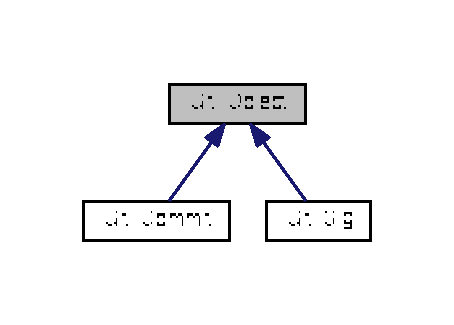
\includegraphics[width=218pt]{class_git_1_1_object__inherit__graph}
\end{center}
\end{figure}
\subsection*{Public Member Functions}
\begin{DoxyCompactItemize}
\item 
std\-::shared\-\_\-ptr$<$ git\-\_\-oid $>$ \hyperlink{class_git_1_1_object_aa517de724dfef848be1cdbde1ccbfa72}{oid} ()
\item 
const std\-::string \hyperlink{class_git_1_1_object_ae8071d40eefb4bab6c54d432b413aebc}{oid\-\_\-str} ()
\end{DoxyCompactItemize}
\subsection*{Protected Member Functions}
\begin{DoxyCompactItemize}
\item 
std\-::shared\-\_\-ptr$<$ git\-\_\-oid $>$ \hyperlink{class_git_1_1_object_a77806dc2a5e3c6f4ba22a280613e0115}{oid} (git\-\_\-oid oid)
\item 
std\-::shared\-\_\-ptr$<$ git\-\_\-oid $>$ \hyperlink{class_git_1_1_object_a4ef40ad77aca900b358713b217f28b0d}{oid} (std\-::string oid)
\end{DoxyCompactItemize}


\subsection{Member Function Documentation}
\hypertarget{class_git_1_1_object_aa517de724dfef848be1cdbde1ccbfa72}{\index{Git\-::\-Object@{Git\-::\-Object}!oid@{oid}}
\index{oid@{oid}!Git::Object@{Git\-::\-Object}}
\subsubsection[{oid}]{\setlength{\rightskip}{0pt plus 5cm}std\-::shared\-\_\-ptr$<$ git\-\_\-oid $>$ Git\-::\-Object\-::oid (
\begin{DoxyParamCaption}
{}
\end{DoxyParamCaption}
)}}\label{class_git_1_1_object_aa517de724dfef848be1cdbde1ccbfa72}
\hypertarget{class_git_1_1_object_a77806dc2a5e3c6f4ba22a280613e0115}{\index{Git\-::\-Object@{Git\-::\-Object}!oid@{oid}}
\index{oid@{oid}!Git::Object@{Git\-::\-Object}}
\subsubsection[{oid}]{\setlength{\rightskip}{0pt plus 5cm}std\-::shared\-\_\-ptr$<$ git\-\_\-oid $>$ Git\-::\-Object\-::oid (
\begin{DoxyParamCaption}
\item[{git\-\_\-oid}]{oid}
\end{DoxyParamCaption}
)\hspace{0.3cm}{\ttfamily [protected]}}}\label{class_git_1_1_object_a77806dc2a5e3c6f4ba22a280613e0115}
\hypertarget{class_git_1_1_object_a4ef40ad77aca900b358713b217f28b0d}{\index{Git\-::\-Object@{Git\-::\-Object}!oid@{oid}}
\index{oid@{oid}!Git::Object@{Git\-::\-Object}}
\subsubsection[{oid}]{\setlength{\rightskip}{0pt plus 5cm}std\-::shared\-\_\-ptr$<$ git\-\_\-oid $>$ Git\-::\-Object\-::oid (
\begin{DoxyParamCaption}
\item[{std\-::string}]{oid}
\end{DoxyParamCaption}
)\hspace{0.3cm}{\ttfamily [protected]}}}\label{class_git_1_1_object_a4ef40ad77aca900b358713b217f28b0d}
\hypertarget{class_git_1_1_object_ae8071d40eefb4bab6c54d432b413aebc}{\index{Git\-::\-Object@{Git\-::\-Object}!oid\-\_\-str@{oid\-\_\-str}}
\index{oid\-\_\-str@{oid\-\_\-str}!Git::Object@{Git\-::\-Object}}
\subsubsection[{oid\-\_\-str}]{\setlength{\rightskip}{0pt plus 5cm}const std\-::string Git\-::\-Object\-::oid\-\_\-str (
\begin{DoxyParamCaption}
{}
\end{DoxyParamCaption}
)}}\label{class_git_1_1_object_ae8071d40eefb4bab6c54d432b413aebc}


The documentation for this class was generated from the following files\-:\begin{DoxyCompactItemize}
\item 
src/\hyperlink{object_8h}{object.\-h}\item 
src/\hyperlink{object_8cpp}{object.\-cpp}\end{DoxyCompactItemize}

\hypertarget{class_git_1_1_repo}{\section{Git\-:\-:Repo Class Reference}
\label{class_git_1_1_repo}\index{Git\-::\-Repo@{Git\-::\-Repo}}
}


{\ttfamily \#include $<$repo.\-h$>$}

\subsection*{Public Member Functions}
\begin{DoxyCompactItemize}
\item 
\hyperlink{class_git_1_1_repo_a7040a7f21faf730376faaa97fecbf59b}{$\sim$\-Repo} ()
\item 
std\-::shared\-\_\-ptr$<$ \hyperlink{class_git_1_1_repo}{Repo} $>$ \hyperlink{class_git_1_1_repo_a1ce0dc274b2a8bf8d78bf2f2627a295d}{clone} (const std\-::string \&\hyperlink{class_git_1_1_repo_a2f1d8cc3ef5c9ca9d57738463e75566a}{path})
\item 
void \hyperlink{class_git_1_1_repo_a2a005418aa8a835d22fac189dcbd3975}{lookup} (const std\-::string \&commit)
\item 
const std\-::string \hyperlink{class_git_1_1_repo_a2f1d8cc3ef5c9ca9d57738463e75566a}{path} ()
\end{DoxyCompactItemize}
\subsection*{Static Public Member Functions}
\begin{DoxyCompactItemize}
\item 
static std\-::shared\-\_\-ptr$<$ \hyperlink{class_git_1_1_repo}{Repo} $>$ \hyperlink{class_git_1_1_repo_a6961faf15258c296804fecd4cefce241}{open} (const std\-::string \&\hyperlink{class_git_1_1_repo_a2f1d8cc3ef5c9ca9d57738463e75566a}{path})
\item 
static std\-::shared\-\_\-ptr$<$ \hyperlink{class_git_1_1_repo}{Repo} $>$ \hyperlink{class_git_1_1_repo_a10fb7c3b59fbeace3e97918df0f3eb71}{open} (git\-\_\-repository $\ast$repo)
\item 
static std\-::shared\-\_\-ptr$<$ \hyperlink{class_git_1_1_repo}{Repo} $>$ \hyperlink{class_git_1_1_repo_a5af0323c729f2387a557095dd43f592e}{init} (const std\-::string \&\hyperlink{class_git_1_1_repo_a2f1d8cc3ef5c9ca9d57738463e75566a}{path}, const bool bare=false)
\item 
static void \hyperlink{class_git_1_1_repo_ae9021cc783b808df5a5f556c7c7af5c7}{clone} (const std\-::string \&url, const std\-::string \&\hyperlink{class_git_1_1_repo_a2f1d8cc3ef5c9ca9d57738463e75566a}{path})
\end{DoxyCompactItemize}


\subsection{Constructor \& Destructor Documentation}
\hypertarget{class_git_1_1_repo_a7040a7f21faf730376faaa97fecbf59b}{\index{Git\-::\-Repo@{Git\-::\-Repo}!$\sim$\-Repo@{$\sim$\-Repo}}
\index{$\sim$\-Repo@{$\sim$\-Repo}!Git::Repo@{Git\-::\-Repo}}
\subsubsection[{$\sim$\-Repo}]{\setlength{\rightskip}{0pt plus 5cm}Git\-::\-Repo\-::$\sim$\-Repo (
\begin{DoxyParamCaption}
{}
\end{DoxyParamCaption}
)}}\label{class_git_1_1_repo_a7040a7f21faf730376faaa97fecbf59b}


\subsection{Member Function Documentation}
\hypertarget{class_git_1_1_repo_a1ce0dc274b2a8bf8d78bf2f2627a295d}{\index{Git\-::\-Repo@{Git\-::\-Repo}!clone@{clone}}
\index{clone@{clone}!Git::Repo@{Git\-::\-Repo}}
\subsubsection[{clone}]{\setlength{\rightskip}{0pt plus 5cm}std\-::shared\-\_\-ptr$<$ {\bf Repo} $>$ Git\-::\-Repo\-::clone (
\begin{DoxyParamCaption}
\item[{const std\-::string \&}]{path}
\end{DoxyParamCaption}
)}}\label{class_git_1_1_repo_a1ce0dc274b2a8bf8d78bf2f2627a295d}
\hypertarget{class_git_1_1_repo_ae9021cc783b808df5a5f556c7c7af5c7}{\index{Git\-::\-Repo@{Git\-::\-Repo}!clone@{clone}}
\index{clone@{clone}!Git::Repo@{Git\-::\-Repo}}
\subsubsection[{clone}]{\setlength{\rightskip}{0pt plus 5cm}static void Git\-::\-Repo\-::clone (
\begin{DoxyParamCaption}
\item[{const std\-::string \&}]{url, }
\item[{const std\-::string \&}]{path}
\end{DoxyParamCaption}
)\hspace{0.3cm}{\ttfamily [static]}}}\label{class_git_1_1_repo_ae9021cc783b808df5a5f556c7c7af5c7}
\hypertarget{class_git_1_1_repo_a5af0323c729f2387a557095dd43f592e}{\index{Git\-::\-Repo@{Git\-::\-Repo}!init@{init}}
\index{init@{init}!Git::Repo@{Git\-::\-Repo}}
\subsubsection[{init}]{\setlength{\rightskip}{0pt plus 5cm}std\-::shared\-\_\-ptr$<$ {\bf Repo} $>$ Git\-::\-Repo\-::init (
\begin{DoxyParamCaption}
\item[{const std\-::string \&}]{path, }
\item[{const bool}]{bare = {\ttfamily false}}
\end{DoxyParamCaption}
)\hspace{0.3cm}{\ttfamily [static]}}}\label{class_git_1_1_repo_a5af0323c729f2387a557095dd43f592e}
\hypertarget{class_git_1_1_repo_a2a005418aa8a835d22fac189dcbd3975}{\index{Git\-::\-Repo@{Git\-::\-Repo}!lookup@{lookup}}
\index{lookup@{lookup}!Git::Repo@{Git\-::\-Repo}}
\subsubsection[{lookup}]{\setlength{\rightskip}{0pt plus 5cm}void Git\-::\-Repo\-::lookup (
\begin{DoxyParamCaption}
\item[{const std\-::string \&}]{commit}
\end{DoxyParamCaption}
)}}\label{class_git_1_1_repo_a2a005418aa8a835d22fac189dcbd3975}
\hypertarget{class_git_1_1_repo_a6961faf15258c296804fecd4cefce241}{\index{Git\-::\-Repo@{Git\-::\-Repo}!open@{open}}
\index{open@{open}!Git::Repo@{Git\-::\-Repo}}
\subsubsection[{open}]{\setlength{\rightskip}{0pt plus 5cm}std\-::shared\-\_\-ptr$<$ {\bf Repo} $>$ Git\-::\-Repo\-::open (
\begin{DoxyParamCaption}
\item[{const std\-::string \&}]{path}
\end{DoxyParamCaption}
)\hspace{0.3cm}{\ttfamily [static]}}}\label{class_git_1_1_repo_a6961faf15258c296804fecd4cefce241}
\hypertarget{class_git_1_1_repo_a10fb7c3b59fbeace3e97918df0f3eb71}{\index{Git\-::\-Repo@{Git\-::\-Repo}!open@{open}}
\index{open@{open}!Git::Repo@{Git\-::\-Repo}}
\subsubsection[{open}]{\setlength{\rightskip}{0pt plus 5cm}std\-::shared\-\_\-ptr$<$ {\bf Repo} $>$ Git\-::\-Repo\-::open (
\begin{DoxyParamCaption}
\item[{git\-\_\-repository $\ast$}]{repo}
\end{DoxyParamCaption}
)\hspace{0.3cm}{\ttfamily [static]}}}\label{class_git_1_1_repo_a10fb7c3b59fbeace3e97918df0f3eb71}
\hypertarget{class_git_1_1_repo_a2f1d8cc3ef5c9ca9d57738463e75566a}{\index{Git\-::\-Repo@{Git\-::\-Repo}!path@{path}}
\index{path@{path}!Git::Repo@{Git\-::\-Repo}}
\subsubsection[{path}]{\setlength{\rightskip}{0pt plus 5cm}const std\-::string Git\-::\-Repo\-::path (
\begin{DoxyParamCaption}
{}
\end{DoxyParamCaption}
)}}\label{class_git_1_1_repo_a2f1d8cc3ef5c9ca9d57738463e75566a}


The documentation for this class was generated from the following files\-:\begin{DoxyCompactItemize}
\item 
src/\hyperlink{repo_8h}{repo.\-h}\item 
src/\hyperlink{repo_8cpp}{repo.\-cpp}\end{DoxyCompactItemize}

\hypertarget{class_git_1_1_sig}{\section{Git\-:\-:Sig Class Reference}
\label{class_git_1_1_sig}\index{Git\-::\-Sig@{Git\-::\-Sig}}
}


{\ttfamily \#include $<$signature.\-h$>$}



Inheritance diagram for Git\-:\-:Sig\-:\nopagebreak
\begin{figure}[H]
\begin{center}
\leavevmode
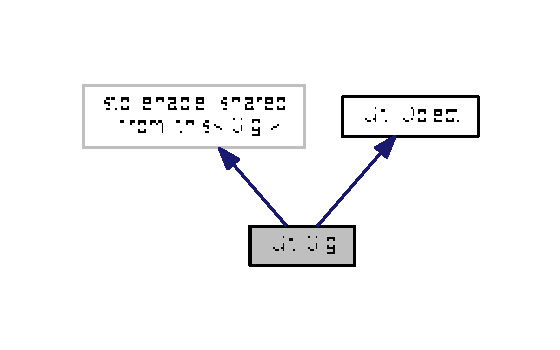
\includegraphics[width=269pt]{class_git_1_1_sig__inherit__graph}
\end{center}
\end{figure}


Collaboration diagram for Git\-:\-:Sig\-:\nopagebreak
\begin{figure}[H]
\begin{center}
\leavevmode
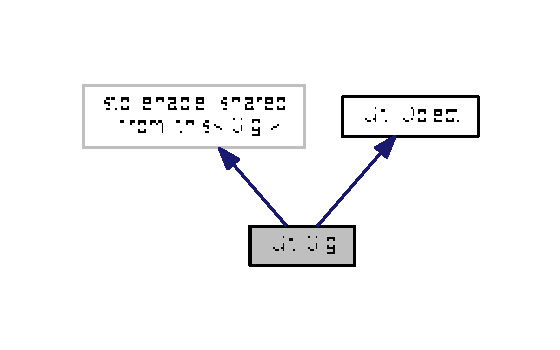
\includegraphics[width=269pt]{class_git_1_1_sig__coll__graph}
\end{center}
\end{figure}
\subsection*{Public Member Functions}
\begin{DoxyCompactItemize}
\item 
\hyperlink{class_git_1_1_sig_abafb1257582300426653b2bb6477bbc2}{$\sim$\-Sig} ()
\item 
git\-\_\-signature $\ast$ \hyperlink{class_git_1_1_sig_aa5f2cf3b7b10a369eb8e62509e4de30e}{ptr} ()
\end{DoxyCompactItemize}
\subsection*{Static Public Member Functions}
\begin{DoxyCompactItemize}
\item 
static std\-::shared\-\_\-ptr$<$ \hyperlink{class_git_1_1_sig}{Sig} $>$ \hyperlink{class_git_1_1_sig_a5166fa376bc02c5052fa75c70470ab45}{create} (std\-::shared\-\_\-ptr$<$ \hyperlink{class_git_1_1_repo}{Repo} $>$ repo)
\end{DoxyCompactItemize}
\subsection*{Additional Inherited Members}


\subsection{Constructor \& Destructor Documentation}
\hypertarget{class_git_1_1_sig_abafb1257582300426653b2bb6477bbc2}{\index{Git\-::\-Sig@{Git\-::\-Sig}!$\sim$\-Sig@{$\sim$\-Sig}}
\index{$\sim$\-Sig@{$\sim$\-Sig}!Git::Sig@{Git\-::\-Sig}}
\subsubsection[{$\sim$\-Sig}]{\setlength{\rightskip}{0pt plus 5cm}Git\-::\-Sig\-::$\sim$\-Sig (
\begin{DoxyParamCaption}
{}
\end{DoxyParamCaption}
)}}\label{class_git_1_1_sig_abafb1257582300426653b2bb6477bbc2}


\subsection{Member Function Documentation}
\hypertarget{class_git_1_1_sig_a5166fa376bc02c5052fa75c70470ab45}{\index{Git\-::\-Sig@{Git\-::\-Sig}!create@{create}}
\index{create@{create}!Git::Sig@{Git\-::\-Sig}}
\subsubsection[{create}]{\setlength{\rightskip}{0pt plus 5cm}std\-::shared\-\_\-ptr$<$ {\bf Sig} $>$ Git\-::\-Sig\-::create (
\begin{DoxyParamCaption}
\item[{std\-::shared\-\_\-ptr$<$ {\bf Repo} $>$}]{repo}
\end{DoxyParamCaption}
)\hspace{0.3cm}{\ttfamily [static]}}}\label{class_git_1_1_sig_a5166fa376bc02c5052fa75c70470ab45}
\hypertarget{class_git_1_1_sig_aa5f2cf3b7b10a369eb8e62509e4de30e}{\index{Git\-::\-Sig@{Git\-::\-Sig}!ptr@{ptr}}
\index{ptr@{ptr}!Git::Sig@{Git\-::\-Sig}}
\subsubsection[{ptr}]{\setlength{\rightskip}{0pt plus 5cm}git\-\_\-signature $\ast$ Git\-::\-Sig\-::ptr (
\begin{DoxyParamCaption}
{}
\end{DoxyParamCaption}
)}}\label{class_git_1_1_sig_aa5f2cf3b7b10a369eb8e62509e4de30e}


The documentation for this class was generated from the following files\-:\begin{DoxyCompactItemize}
\item 
src/\hyperlink{signature_8h}{signature.\-h}\item 
src/\hyperlink{signature_8cpp}{signature.\-cpp}\end{DoxyCompactItemize}

\chapter{File Documentation}
\hypertarget{commit_8cpp}{\section{src/commit.cpp File Reference}
\label{commit_8cpp}\index{src/commit.\-cpp@{src/commit.\-cpp}}
}
{\ttfamily \#include \char`\"{}repo.\-h\char`\"{}}\\*
{\ttfamily \#include \char`\"{}commit.\-h\char`\"{}}\\*
{\ttfamily \#include \char`\"{}exception.\-h\char`\"{}}\\*
{\ttfamily \#include \char`\"{}object.\-h\char`\"{}}\\*
Include dependency graph for commit.\-cpp\-:\nopagebreak
\begin{figure}[H]
\begin{center}
\leavevmode
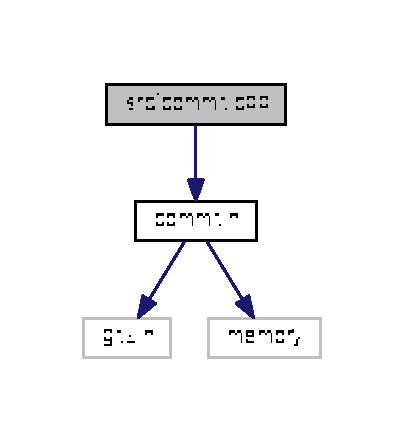
\includegraphics[width=350pt]{commit_8cpp__incl}
\end{center}
\end{figure}
\subsection*{Namespaces}
\begin{DoxyCompactItemize}
\item 
\hyperlink{namespace_git}{Git}
\begin{DoxyCompactList}\small\item\em libgit++ \end{DoxyCompactList}\end{DoxyCompactItemize}

\hypertarget{commit_8h}{\section{src/commit.h File Reference}
\label{commit_8h}\index{src/commit.\-h@{src/commit.\-h}}
}
{\ttfamily \#include $<$git2.\-h$>$}\\*
{\ttfamily \#include $<$memory$>$}\\*
{\ttfamily \#include \char`\"{}repo.\-h\char`\"{}}\\*
{\ttfamily \#include \char`\"{}object.\-h\char`\"{}}\\*
{\ttfamily \#include \char`\"{}signature.\-h\char`\"{}}\\*
Include dependency graph for commit.\-h\-:\nopagebreak
\begin{figure}[H]
\begin{center}
\leavevmode
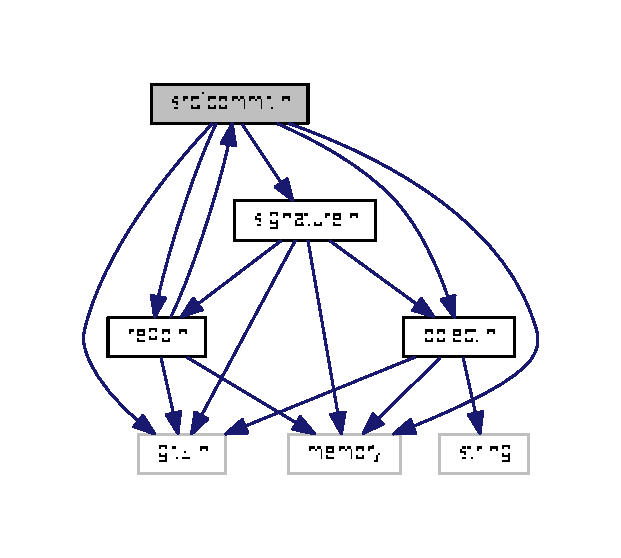
\includegraphics[width=298pt]{commit_8h__incl}
\end{center}
\end{figure}
This graph shows which files directly or indirectly include this file\-:\nopagebreak
\begin{figure}[H]
\begin{center}
\leavevmode
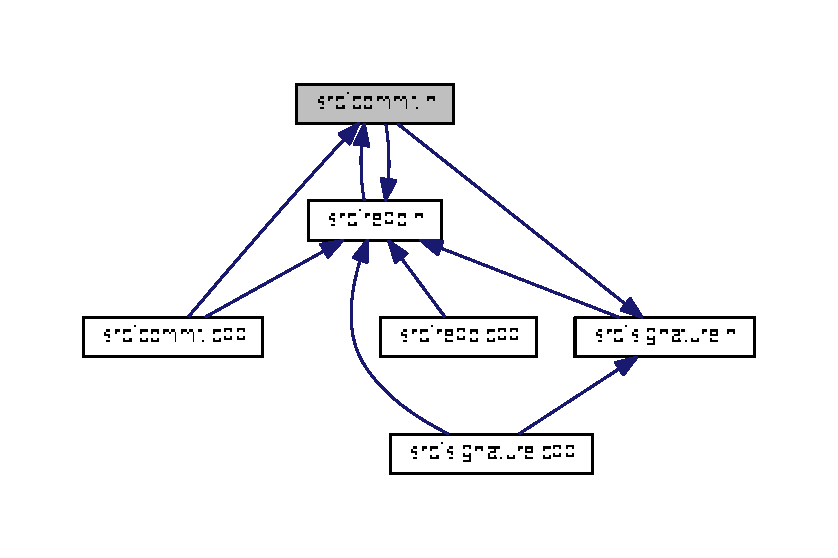
\includegraphics[width=350pt]{commit_8h__dep__incl}
\end{center}
\end{figure}
\subsection*{Classes}
\begin{DoxyCompactItemize}
\item 
class \hyperlink{class_git_1_1_commit}{Git\-::\-Commit}
\end{DoxyCompactItemize}
\subsection*{Namespaces}
\begin{DoxyCompactItemize}
\item 
\hyperlink{namespace_git}{Git}
\begin{DoxyCompactList}\small\item\em libgit++ \end{DoxyCompactList}\end{DoxyCompactItemize}

\hypertarget{exception_8cpp}{\section{src/exception.cpp File Reference}
\label{exception_8cpp}\index{src/exception.\-cpp@{src/exception.\-cpp}}
}
{\ttfamily \#include \char`\"{}exception.\-h\char`\"{}}\\*
Include dependency graph for exception.\-cpp\-:\nopagebreak
\begin{figure}[H]
\begin{center}
\leavevmode
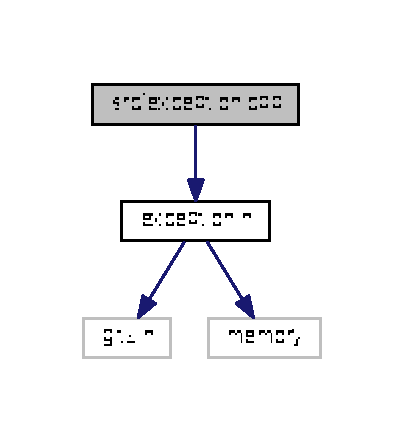
\includegraphics[width=194pt]{exception_8cpp__incl}
\end{center}
\end{figure}
\subsection*{Namespaces}
\begin{DoxyCompactItemize}
\item 
\hyperlink{namespace_git}{Git}
\begin{DoxyCompactList}\small\item\em libgit++ \end{DoxyCompactList}\end{DoxyCompactItemize}
\subsection*{Functions}
\begin{DoxyCompactItemize}
\item 
void \hyperlink{namespace_git_a278e75304a5420da6ca1611ce9ffddc0}{Git\-::\-Throw} (const int \&error)
\end{DoxyCompactItemize}

\hypertarget{exception_8h}{\section{src/exception.h File Reference}
\label{exception_8h}\index{src/exception.\-h@{src/exception.\-h}}
}
{\ttfamily \#include $<$git2.\-h$>$}\\*
{\ttfamily \#include $<$memory$>$}\\*
Include dependency graph for exception.\-h\-:
\nopagebreak
\begin{figure}[H]
\begin{center}
\leavevmode
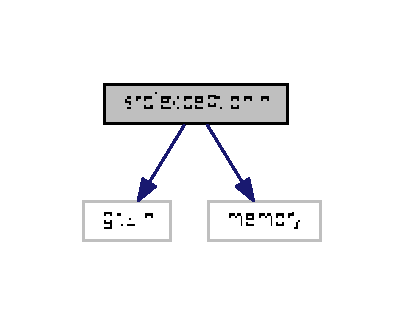
\includegraphics[width=194pt]{exception_8h__incl}
\end{center}
\end{figure}
This graph shows which files directly or indirectly include this file\-:
\nopagebreak
\begin{figure}[H]
\begin{center}
\leavevmode
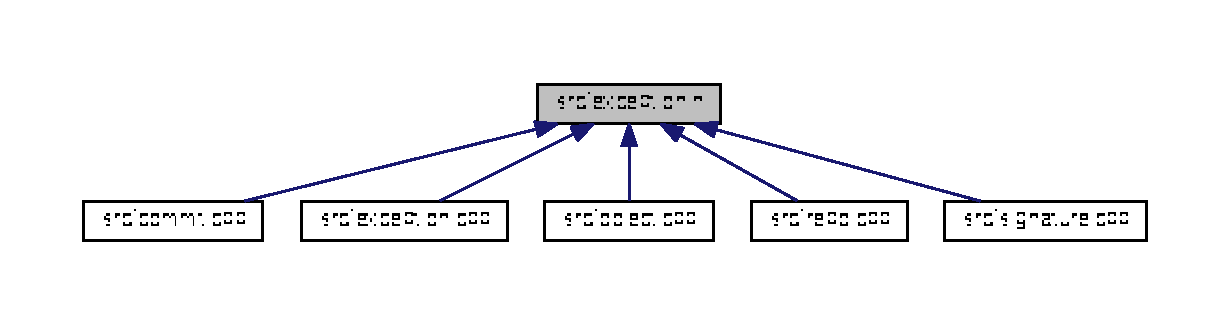
\includegraphics[width=271pt]{exception_8h__dep__incl}
\end{center}
\end{figure}
\subsection*{Classes}
\begin{DoxyCompactItemize}
\item 
class \hyperlink{class_git_1_1_exception}{Git\-::\-Exception}
\end{DoxyCompactItemize}
\subsection*{Namespaces}
\begin{DoxyCompactItemize}
\item 
\hyperlink{namespace_git}{Git}
\end{DoxyCompactItemize}
\subsection*{Functions}
\begin{DoxyCompactItemize}
\item 
void \hyperlink{namespace_git_a278e75304a5420da6ca1611ce9ffddc0}{Git\-::\-Throw} (const int \&error)
\end{DoxyCompactItemize}

\hypertarget{object_8cpp}{\section{src/object.cpp File Reference}
\label{object_8cpp}\index{src/object.\-cpp@{src/object.\-cpp}}
}
{\ttfamily \#include \char`\"{}object.\-h\char`\"{}}\\*
{\ttfamily \#include \char`\"{}exception.\-h\char`\"{}}\\*
Include dependency graph for object.\-cpp\-:\nopagebreak
\begin{figure}[H]
\begin{center}
\leavevmode
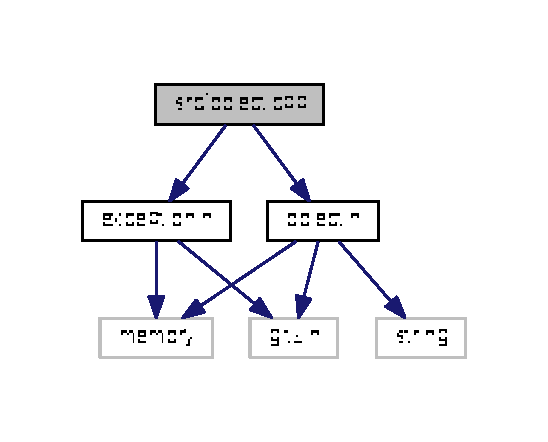
\includegraphics[width=263pt]{object_8cpp__incl}
\end{center}
\end{figure}
\subsection*{Namespaces}
\begin{DoxyCompactItemize}
\item 
\hyperlink{namespace_git}{Git}
\begin{DoxyCompactList}\small\item\em libgit++ \end{DoxyCompactList}\end{DoxyCompactItemize}
\subsection*{Functions}
\begin{DoxyCompactItemize}
\item 
git\-\_\-oid \hyperlink{namespace_git_a20e639531f5c04252e0ce86622c2e77e}{Git\-::oid} (const std\-::string \&sha)
\item 
const std\-::string \hyperlink{namespace_git_a7058573edae76cc2fbafcfe04e13dabc}{Git\-::oid} (git\-\_\-oid \&oid)
\end{DoxyCompactItemize}

\hypertarget{object_8h}{\section{src/object.h File Reference}
\label{object_8h}\index{src/object.\-h@{src/object.\-h}}
}
{\ttfamily \#include $<$git2.\-h$>$}\\*
{\ttfamily \#include $<$string$>$}\\*
{\ttfamily \#include $<$memory$>$}\\*
Include dependency graph for object.\-h\-:\nopagebreak
\begin{figure}[H]
\begin{center}
\leavevmode
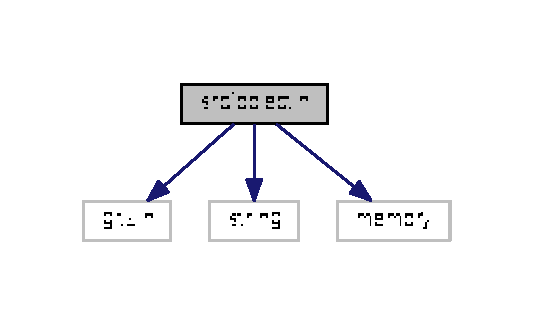
\includegraphics[width=256pt]{object_8h__incl}
\end{center}
\end{figure}
This graph shows which files directly or indirectly include this file\-:\nopagebreak
\begin{figure}[H]
\begin{center}
\leavevmode
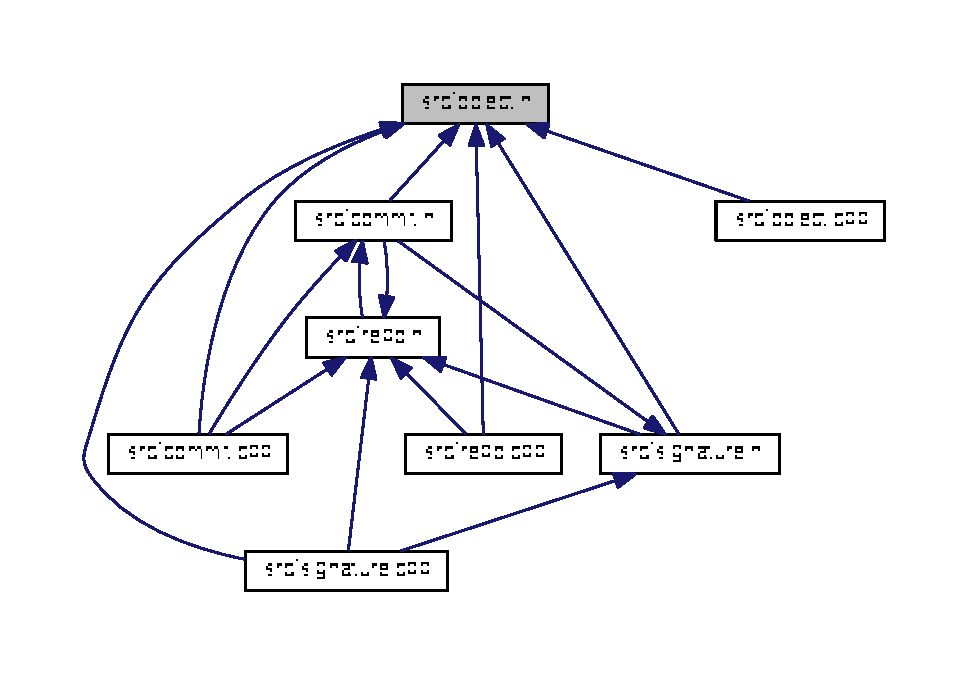
\includegraphics[width=350pt]{object_8h__dep__incl}
\end{center}
\end{figure}
\subsection*{Classes}
\begin{DoxyCompactItemize}
\item 
class \hyperlink{class_git_1_1_object}{Git\-::\-Object}
\end{DoxyCompactItemize}
\subsection*{Namespaces}
\begin{DoxyCompactItemize}
\item 
\hyperlink{namespace_git}{Git}
\begin{DoxyCompactList}\small\item\em libgit++ \end{DoxyCompactList}\end{DoxyCompactItemize}
\subsection*{Functions}
\begin{DoxyCompactItemize}
\item 
git\-\_\-oid \hyperlink{namespace_git_a20e639531f5c04252e0ce86622c2e77e}{Git\-::oid} (const std\-::string \&sha)
\item 
const std\-::string \hyperlink{namespace_git_a7058573edae76cc2fbafcfe04e13dabc}{Git\-::oid} (git\-\_\-oid \&oid)
\end{DoxyCompactItemize}

\hypertarget{repo_8cpp}{\section{src/repo.cpp File Reference}
\label{repo_8cpp}\index{src/repo.\-cpp@{src/repo.\-cpp}}
}
{\ttfamily \#include \char`\"{}exception.\-h\char`\"{}}\\*
{\ttfamily \#include \char`\"{}repo.\-h\char`\"{}}\\*
{\ttfamily \#include \char`\"{}object.\-h\char`\"{}}\\*
Include dependency graph for repo.\-cpp\-:\nopagebreak
\begin{figure}[H]
\begin{center}
\leavevmode
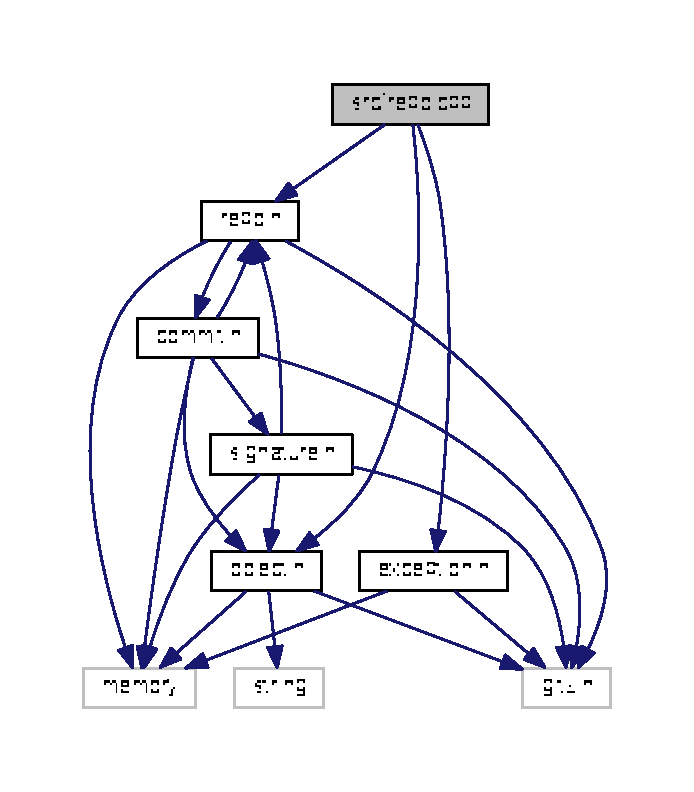
\includegraphics[width=333pt]{repo_8cpp__incl}
\end{center}
\end{figure}
\subsection*{Namespaces}
\begin{DoxyCompactItemize}
\item 
\hyperlink{namespace_git}{Git}
\begin{DoxyCompactList}\small\item\em libgit++ \end{DoxyCompactList}\end{DoxyCompactItemize}

\hypertarget{repo_8h}{\section{src/repo.h File Reference}
\label{repo_8h}\index{src/repo.\-h@{src/repo.\-h}}
}


Manage repository.  


{\ttfamily \#include $<$git2.\-h$>$}\\*
{\ttfamily \#include $<$memory$>$}\\*
{\ttfamily \#include \char`\"{}commit.\-h\char`\"{}}\\*
Include dependency graph for repo.\-h\-:\nopagebreak
\begin{figure}[H]
\begin{center}
\leavevmode
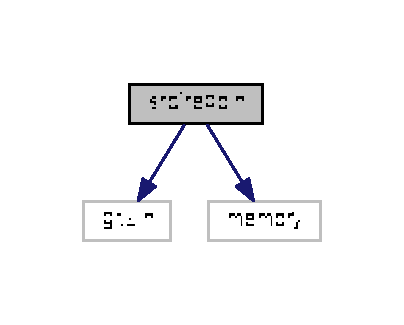
\includegraphics[width=285pt]{repo_8h__incl}
\end{center}
\end{figure}
This graph shows which files directly or indirectly include this file\-:\nopagebreak
\begin{figure}[H]
\begin{center}
\leavevmode
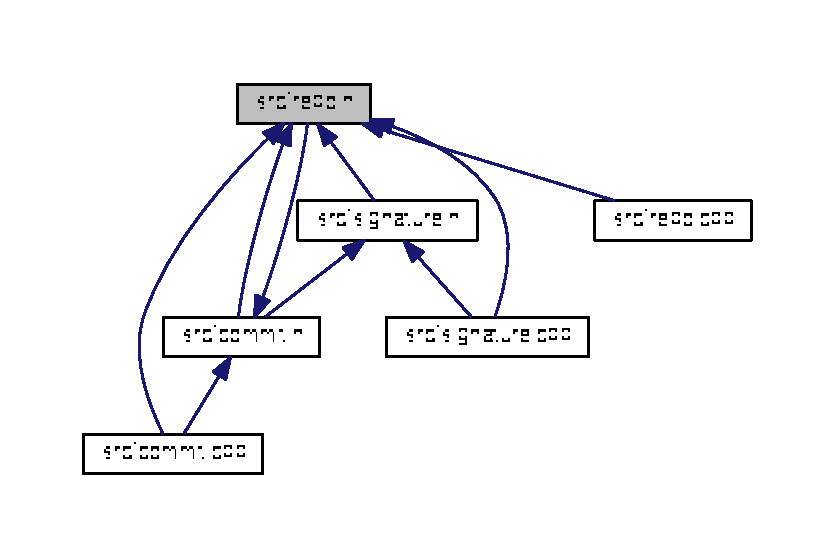
\includegraphics[width=350pt]{repo_8h__dep__incl}
\end{center}
\end{figure}
\subsection*{Classes}
\begin{DoxyCompactItemize}
\item 
class \hyperlink{class_git_1_1_repo}{Git\-::\-Repo}
\begin{DoxyCompactList}\small\item\em Manage repository. \end{DoxyCompactList}\end{DoxyCompactItemize}
\subsection*{Namespaces}
\begin{DoxyCompactItemize}
\item 
\hyperlink{namespace_git}{Git}
\begin{DoxyCompactList}\small\item\em libgit++ \end{DoxyCompactList}\end{DoxyCompactItemize}


\subsection{Detailed Description}
Manage repository. \begin{DoxyAuthor}{Author}
Adrien Jeser \href{mailto:adrien@jeser.me}{\tt adrien@jeser.\-me} 
\end{DoxyAuthor}

\hypertarget{signature_8cpp}{\section{src/signature.cpp File Reference}
\label{signature_8cpp}\index{src/signature.\-cpp@{src/signature.\-cpp}}
}
{\ttfamily \#include \char`\"{}repo.\-h\char`\"{}}\\*
{\ttfamily \#include \char`\"{}signature.\-h\char`\"{}}\\*
{\ttfamily \#include \char`\"{}exception.\-h\char`\"{}}\\*
{\ttfamily \#include \char`\"{}object.\-h\char`\"{}}\\*
Include dependency graph for signature.\-cpp\-:\nopagebreak
\begin{figure}[H]
\begin{center}
\leavevmode
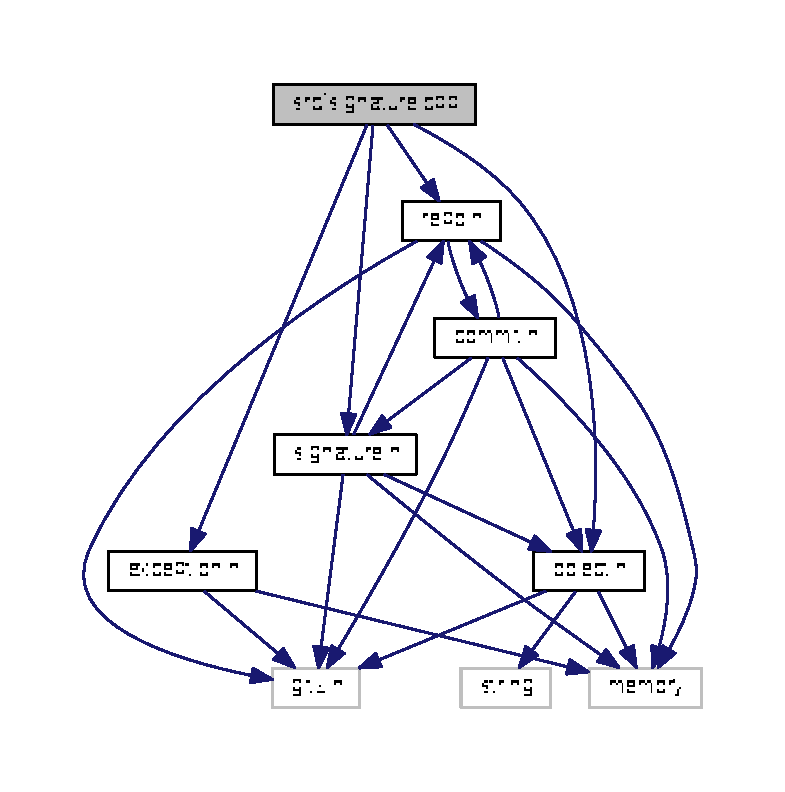
\includegraphics[width=350pt]{signature_8cpp__incl}
\end{center}
\end{figure}
\subsection*{Namespaces}
\begin{DoxyCompactItemize}
\item 
\hyperlink{namespace_git}{Git}
\begin{DoxyCompactList}\small\item\em libgit++ \end{DoxyCompactList}\end{DoxyCompactItemize}

\hypertarget{signature_8h}{\section{src/signature.h File Reference}
\label{signature_8h}\index{src/signature.\-h@{src/signature.\-h}}
}
{\ttfamily \#include $<$git2.\-h$>$}\\*
{\ttfamily \#include $<$memory$>$}\\*
{\ttfamily \#include \char`\"{}repo.\-h\char`\"{}}\\*
{\ttfamily \#include \char`\"{}object.\-h\char`\"{}}\\*
Include dependency graph for signature.\-h\-:\nopagebreak
\begin{figure}[H]
\begin{center}
\leavevmode
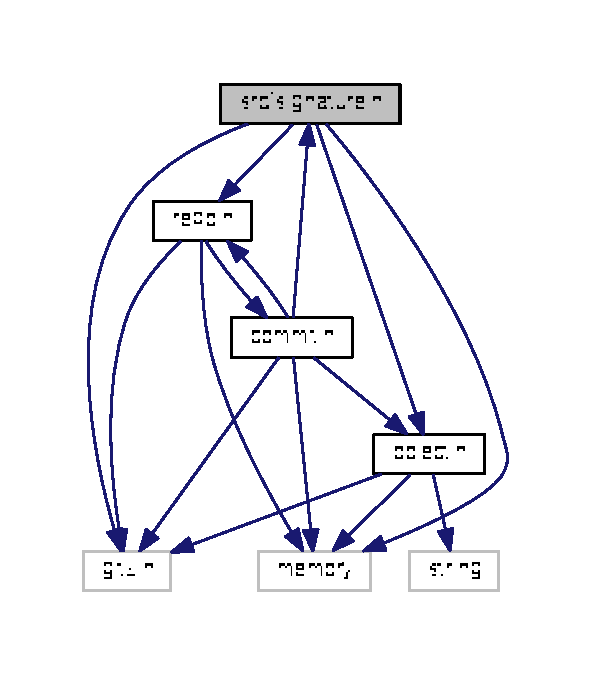
\includegraphics[width=284pt]{signature_8h__incl}
\end{center}
\end{figure}
This graph shows which files directly or indirectly include this file\-:\nopagebreak
\begin{figure}[H]
\begin{center}
\leavevmode
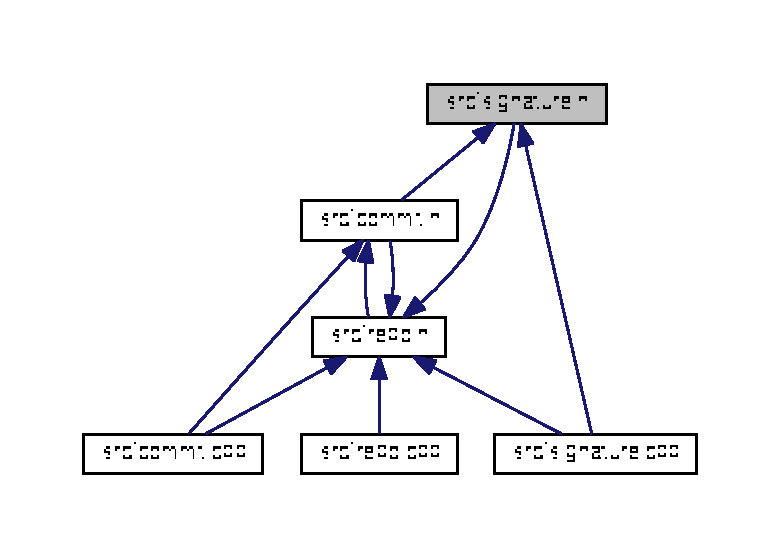
\includegraphics[width=350pt]{signature_8h__dep__incl}
\end{center}
\end{figure}
\subsection*{Classes}
\begin{DoxyCompactItemize}
\item 
class \hyperlink{class_git_1_1_sig}{Git\-::\-Sig}
\end{DoxyCompactItemize}
\subsection*{Namespaces}
\begin{DoxyCompactItemize}
\item 
\hyperlink{namespace_git}{Git}
\begin{DoxyCompactList}\small\item\em libgit++ \end{DoxyCompactList}\end{DoxyCompactItemize}

%--- End generated contents ---

% Index
\newpage
\phantomsection
\addcontentsline{toc}{chapter}{Index}
\printindex

\end{document}
